%!TEX root = ../Electrodynamics.tex
\subsection{\textcolor{red}{ПУСТО} Медленные волны, направляемые плоским диэлектрическим слоем...}


\subsection{\textcolor{red}{МИНИМУМ} Главные (ТЕМ) волны в линиях передач. Условие существования ТЕМ волны. ТЕМ волна в коаксиальной линии
(Картинка силовых линий, зависимость полей от координат).}
Главные (TEM) волны в линиях передачи с идеальными границами

У TEM-волн поперечное волновое число $\varkappa=0$:
\begin{equation*}
\varkappa=0 \Rightarrow h=k= \frac{\omega}{c}\sqrt{\varepsilon \mu}
\end{equation*}
Поля таких волн выражаются следующим образом через функцию $\varphi$:
\begin{gather*}
\label{eperp}
\vec{E}_\perp=-\frac{1}{\sqrt{\varepsilon \mu}}\nabla_\perp \varphi\\
\vec{H}_\perp=-\frac{1}{\mu}\qty[\nabla_\perp \varphi,\vec{z}_0]
\end{gather*}

При этом выполняются \textbf{граничные условия}: на каждом из проводников (допустим, есть набор проводников, вдоль которых распространяется волна)
\begin{equation*}
\varphi|_{l_i}=C_i,
\end{equation*}
причем константа не обязана быть одна для всех проводников.

\begin{figure}[h!]
	\centering
	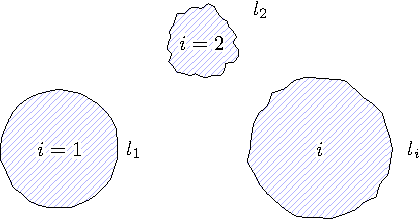
\includegraphics[scale=1]{img/lect4_ris1}
	\caption{Набор проводников в задаче}
	\label{fig:lect4:1}
\end{figure}

\textbf{Внутренняя задача}

\begin{figure}[h!]
	\centering
	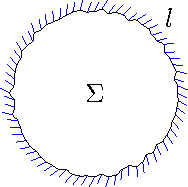
\includegraphics[scale=1]{img/lect4_ris2}
	\caption{Случай одного проводника}
	\label{fig:lect4:2}
\end{figure}
Пусть у нас есть только один проводник, в котором есть цилиндрическая полость (рис. \ref{fig:lect4:2}). Рассмотрим внутреннюю задачу, т.е. распространение волны внутри цилиндрической полости. Оказывается, для граничного условия $\varphi_\perp|_l=C_1$ существует только тривиальное решение $\varphi_\perp=C_1$. Для доказательства необходимо воспользоваться теоремой и минимуме и максимуме для гармонической функции.
%\begin{equation*}
%\Delta \varphi=\Div\qty(\varphi\nabla \varphi)=0 \quad \bigg| \iint\limits_\Sigma
%\end{equation*}
%Это такая задача, которую проще доказать самому. Попробуйте это сделать сами.

\textbf{Внешняя задача}

Зададимся вопросом о решении той же задачи:
\begin{equation*}
\Delta_\perp \varphi=0, \quad \varphi|_l=\mathrm{const}
\end{equation*}
Только теперь будем рассматривать её в области вне проводника

Для начала рассмотрим задачу попроще, поле нити (рис. \ref{fig:lect4:3}). Её решение известно:
\begin{equation*}
\Delta_\perp \varphi=0 
\quad \Rightarrow \quad
\varphi \sim \ln r
\end{equation*} 

Характер убывания полей здесь $\displaystyle E_r\sim \frac{1}{r}$, а для магнитного поля в силу импедансного соотношения
$\displaystyle\frac{E_r}{H_\phi}=\eta_{\perp\text{в}}=1, \quad H_\varphi\sim\frac{1}{r}$:
\begin{equation*}
E_r=H_\phi\sim\frac{1}{r}
\end{equation*}
\begin{figure}[h!]
	\centering
	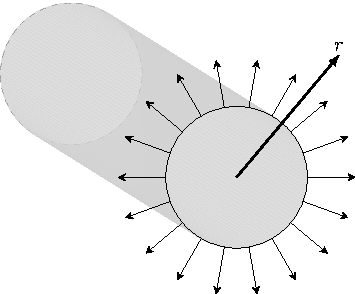
\includegraphics[width =0.4\linewidth]{img/lect4_ris3}
	\caption{Поле бесконечной проводящей нити}
	\label{fig:lect4:3}
\end{figure}

Посмотрим на поведение полей при $r\to\infty$. Говорят, нужно поставить граничные условия (или закон убывания) на
бесконечности. Чем плох закон $\frac{1}{r}$?

Посчитаем средний по времени поток энергии через поперечное сечение, в котором распространяется волна. Сечение
бесконечно, за исключением конечной площади проводника.

Сначала вычислим вектор Пойнтинга (средний по времени и в проекции на $z$):
\begin{equation*}
\overline{S}_z=\frac{c}{8 \pi}\mathrm{Re}\qty(E_r\cdot H_\phi^*)\sim\frac{1}{r^2}
\end{equation*}
\begin{equation*}
\Pi=\iint\limits_\Sigma \overline{S}_z ds \sim
\iint\limits_\Sigma \frac{1}{r^2} (2\pi r \dd{r})
\sim \int\limits_a^\infty = \ln\frac{\infty}{a}=\infty
\end{equation*}
Интеграл расходится на бесконечности. Говорят, что расходимость носит логарифмический характер. Получили бесконечную мощность волны: такую волну невозможно создать реальным источником --- волна не удовлетворяет критерию энергетической реализуемости.

Можно сделать важный вывод: \textbf{вдоль одиночного проводника TEM-волна с конечной энергией распространятся не может}. Распространение возможно, если количество проводников будет больше одного. Например, в линии из двух проводников (рис. \ref{fig:lect4:4}) TEM-волна уже возможна.

\begin{figure}[h!]
	\centering
	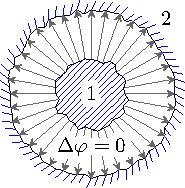
\includegraphics[scale=1.5]{img/lect4_ris4}
	\caption{Закрытая линия из двух проводников}
	\label{fig:lect4:4}
\end{figure}

Можно модифицировать задачу с нитью (рис. \ref{fig:lect4:5}):

\begin{figure}[h!]
	\centering
	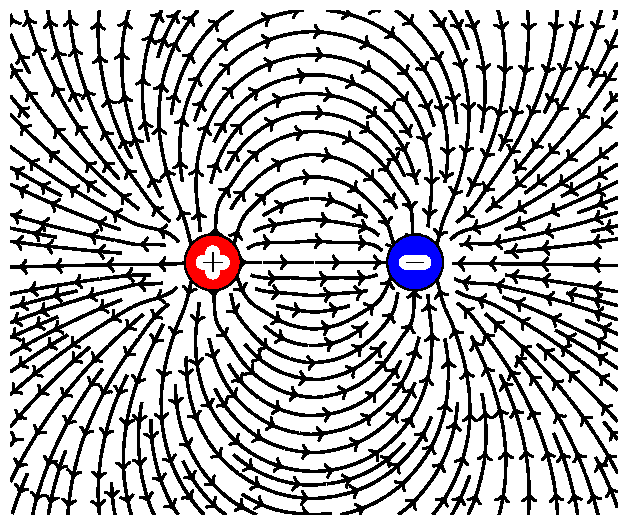
\includegraphics[scale=0.7]{img/lect4_ris5}
	\caption{Поле двухпроводной линии}
	\label{fig:lect4:5}
\end{figure}

В поперечном разрезе это поле диполя, а оно спадает быстрее, $\sim \frac{1}{r^2}$. Тогда
\begin{equation*}
E_\perp\sim H_\perp \sim \frac{1}{r^2}
\quad \Rightarrow \quad
\overline{S}_z \sim \frac{1}{r^4}, \quad
\Pi \sim \int\limits_{L_\text{характ}}^\infty \frac{1}{r^3} \dd{r}
\end{equation*}

Мощность волны конечна, значит, в модифицированной задаче TEM-волна энергетически реализуема.

\textbf{Конечный вывод:} TEM-волна в идеальной линии передачи возможна, если число проводников $\geq 2$.

Например, в коаксиальной линии (рис. \ref{fig:lect4:6}) TEM-волна возможна.

\begin{figure}[h!]
	\centering
	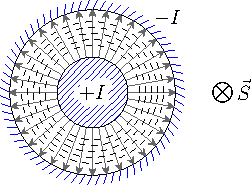
\includegraphics[scale=1.5]{img/lect4_ris6}
	\caption{Поле в коаксиальном кабеле}
	\label{fig:lect4:6}
\end{figure}

Зададимся вопросом: возможны ли в такой линии TE и TM волны? Сформулируем утверждение, пока без доказательства:
\textbf{в открытых линиях передачи TE и TM волны не существуют}.
